\section{Round trip in Bali}

Date: 14/04/2008

\begin{multicols}{2}

Oulala... que de choses a dire...

Je vous ai laissés à la fin de ma première semaine à Bali. Ma deuxième semaine à été très mouvementée, car j'ai loué un scooter pour faire un tour de l'ile, en 4 jours.

Me voila donc parti sur les routes, avec pour seule carte un plan de l'ile qui tiendrais presque sur une seule main, sur laquelle figure les grandes routes, pour les reste, la discussion avec les gens m'a bien suffit à m'orienter.

Alors premiere precision : parlons de la circulation ici... Nous vous avions parlé avec Cécile de la circulation en Inde, je n'aurais jamais loué une scooter en Inde, trop dangereux pour un novice. Ici c'est différent... quoi que... Les intersections sont respectées, les feux aussi, mais par contre il faut savoir qu'il y a réellement deux types de circulations qui cohabitent ici : les voitures qui font ce qu'elle peuvent pour respecter le code de la route, ce qui ne les empêchent pas de s'arrêter en plein virage et au milieu de la route sur ce que l'on appelerait une route départementale. Et les 2 roues, qui font ce qu'ils veulent : On peut doubler par la gauche, par la droite, slalomer, rouler à contre sens... don't worry, be happy. De temps en temps ça a du bon d'être en deux roues...

Mais que fait la police !!! Réponse : elle encaisse les backchiches. On a beaucoup plus de chances de se faire arrêter ici quand on est "western" (blanc) que quand on est Indonésien. Pourquoi ? Parce qu'on est plus solvable bien sûr... La majorité du temps le seul et unique but du policier qui vous arrête est que vous lui donniez un billet, on peut rouler sans permis ici, du moment qu'on a 50.000 Rp en poche. Quand je parle de contrôle je ne dis pas ça en l'air, je me suis fait contrôlé trois fois ce soir même sur une zone de moins de 50m de diamètre, sans éxagérer, mais je n'ai pas eu a sortir de billets, j'étais (presque) en règle.

Nous fermons la parenthèse code la route pour cette fois-ci.

\hspace*{-0.65cm}
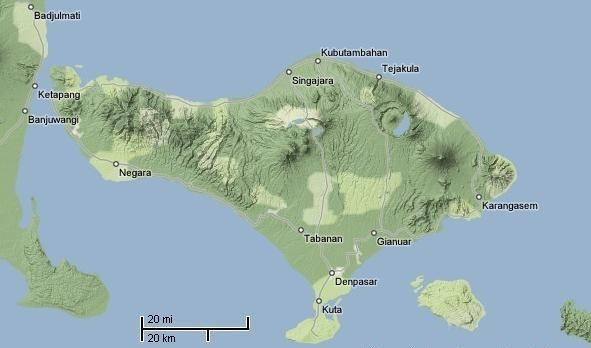
\includegraphics[width=4.8cm]{articles/Round-trip-in-bali/1208257310r6gK.jpg}
Carte de Bali.


Le premier jour je suis allé dans un coin de surfers, en dessous de Tabanan, cette journée a surtout été pour moi la découverte avec la conduite indonésienne, à gauche, et son code de la route folklorique. Le soir je me suis posé à une terrasse, à discuter, je suis tombé sur des Français. Enfin quand je dis Francais, c'est d'origine, car ils voyagent tellement qu'ils n'ont jamais vu la couleur d'un euro ! La vie est belle quand on se contente de trois sous pour vivre, et ainsi voyager partout dans le monde.

Le lendemain, remontée sur Singaraja à travers de magnifiques rizières, c'est un coup à avoir un accident tellement je tournais la tete pour voir les superbes paysages qui défilaient.

\hspace*{-0.65cm}
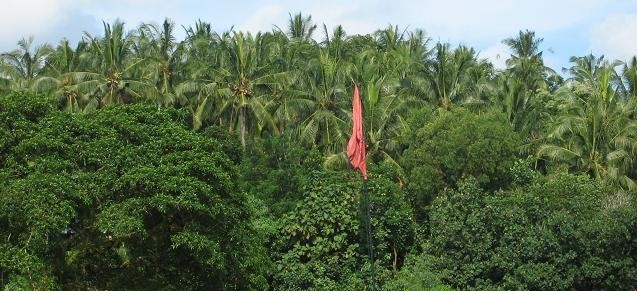
\includegraphics[width=4.8cm]{articles/Round-trip-in-bali/1208257309URc4.jpg}
Cocotiers sur la route.


\hspace*{-0.65cm}
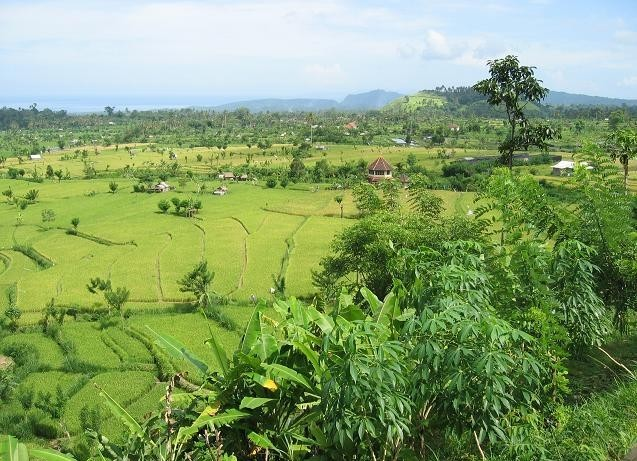
\includegraphics[width=4.8cm]{articles/Round-trip-in-bali/1208257304SP22.jpg}
Rizières.


\hspace*{-0.65cm}
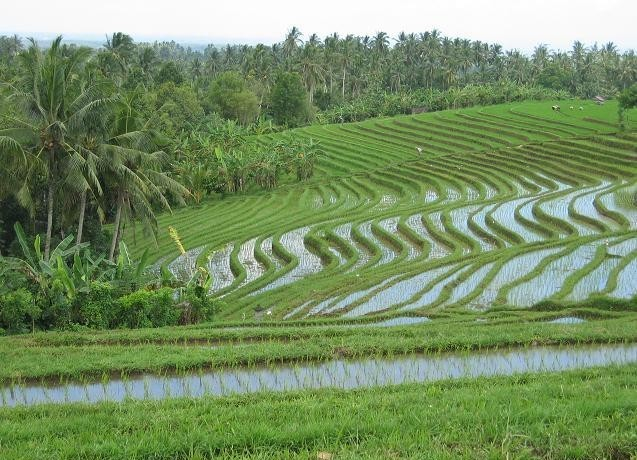
\includegraphics[width=4.8cm]{articles/Round-trip-in-bali/1208257308isJF.jpg}
D'autres rizières.


\hspace*{-0.65cm}
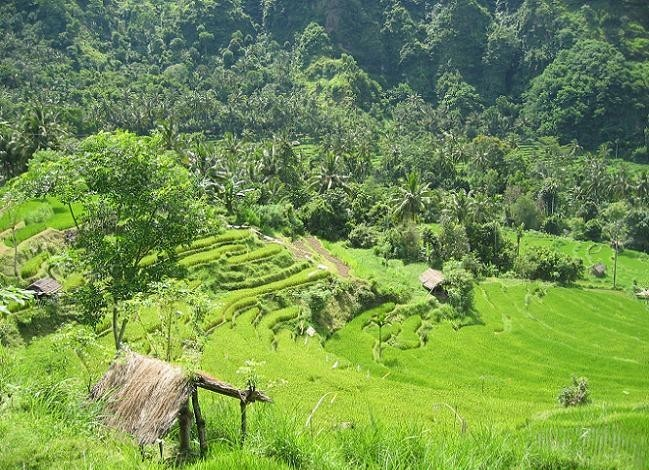
\includegraphics[width=4.8cm]{articles/Round-trip-in-bali/1208257307G9b6.jpg}
Et encore des rizières :)

Quand j'ai pris cette photo, il y avait un bruit au loin, j'ai mis du temps à comprendre qu'il s'agissait d'un homme, dans la cabane du bas, qui me faisait signe, et qui faisait du bruit pour que je le remarque. Un signe de ma part et il s'en est retourné dans sa cabane, il a du penser qu'il serait sur la photos. Les gens ici sont aussi tellement gentils que l'on a vraiment envie de leur faire plaisir.

Singaraja : pour sur ce n'est pas la meilleure étape, coin touristique si il en est, j'ai quand même réussi à me trouver un petit endroit à l'écart pour dormir, mais c'était assez difficile car, ne voulant pas paraître comme ignorant quand on leur pose une question, les gens ici vous repondront toujours une direction et une distance lorsque vous cherchez un "cheap hôtel", le tout étant apres de savoir si ce que l'on vous a dit est vrai ou pas. Il m'est arrivé que l'on me réponde alors que la personne ne parlait pas anglais, et n'avait donc pas compris la question.

Apres Singaraja, direction Seraya, au bout de la pointe de Karangasem. Je suis allé dormir chez Sales, amis de Patrick, qui m'a accueilli comme un roi, nous avons passé une super soirée avec sa famille et ses amis à boire un coup.

Sales et l'un de ses deux fils, qui a adoré les séances de guilis prodigués par mes soins.

\hspace*{-0.65cm}
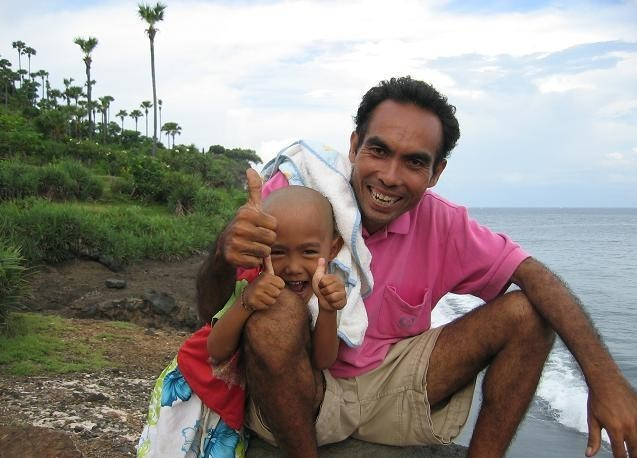
\includegraphics[width=4.8cm]{articles/Round-trip-in-bali/1208257303gr5r.jpg}
Sales et son fils Edi.

Et vous savez quoi... ? j'ai eu un super petit dej le lendemain matin, une noix de coco qui était encore à 15m de haut 10 minutes avant que je boive son jus... si c'est pas la classe...

\hspace*{-0.65cm}
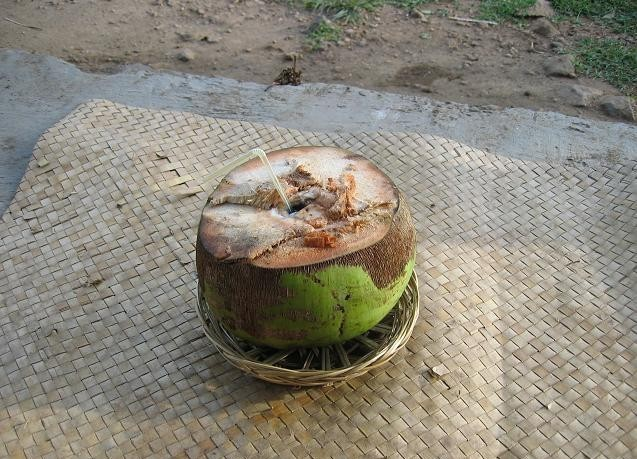
\includegraphics[width=4.8cm]{articles/Round-trip-in-bali/1208257299a93l.jpg}
Mon p'tit dej'


Je suis redescendu de Seraya avec Sales en scooter, puis, en repartant demain, nous le déposerons près de chez lui après environs 7 heures de voile.

C'est maintenant les opérations de remplissage des soutes, avec de l'eau, du carburant, et de la nourritures. Puis dire au revoir, surtout pour Patrick qui a été ici durant 7 mois. De mon coté aussi c'est un peu dur de partir, il y a déjà des personnes que j'aimerais revoir.

Direction Madura, sur l'île de Java pour les jours à venir, puis Bornéo, plus au nord. Et de Bornéo nous mettrons le cap sur Singapour, où je dois arriver avant la fin de mon visa Indonésien (fin du mois d'avril).

Voila, j'éspère que suivre mon voyage vous plaît toujours, je vous dis à très bientôt.

\end{multicols}

\bigskip
\textbf{\textsc{Commentaires}}

\medskip
Mamam titou a écrit le 14 avril 2008 :
\begin{displayquote}
Ton pote t'a traité de salopard - je ne fais pas de  délation mais je l'ai bien entendu - comme d'hab les photos sont superbes - profites de ton séjour nautique tu es dans ton élément. bon courage et je pense que nous aurons l'occasion de nous revoir sur la région parisienne... Gros bisous de la famille titou.
\end{displayquote}

\medskip
Cécile a écrit le 14 avril 2008 :
\begin{displayquote}
Magnifique! que dire de plus...
\end{displayquote}

\medskip
Zan a écrit le 14 avril 2008 :
\begin{displayquote}
Yo!
Lors de mon ST40, j'ai des potes qui sont partis à Bali et qui ont profité de Bali. C'était effectivement un peu des paysages dans le même genre sur leurs photos... Ma-Gnin-Fi-Que!
Profites veinard! :p
\end{displayquote}

\medskip
Jaco a écrit le 15 avril 2008 :
\begin{displayquote}
Mouais ya beaucoup de vert quoi... C'est comme en Alsace, sauf que c'est pas du vert mais du gris, surtout dans le ciel.
Bonne continuation !
\end{displayquote}

\medskip
Peggy a écrit le 16 avril 2008 :
\begin{displayquote}
Coucou!
Et question alimentaire (même l'eau), aucun risque ?
Bizx.
\end{displayquote}

\medskip
Anick a écrit le 17 avril 2008 :
\begin{displayquote}
Etienne...
\end{displayquote}

\medskip
Monique et Alain a écrit le 17 avril 2008 :
\begin{displayquote}
Nous comprenons ton enthousiasme à découvrir encore de nouvelles contrées, de nouvelles cultures! Soit prudent et bon vent pour ta traversée, évite les pirates du Détroit de Malacca!
\end{displayquote}

\medskip
Etienne a écrit le 22 avril 2008 :
\begin{displayquote}
Héhé... et bien je vois que les commentaires marchent bien.
Je suis actuellement à Kumai (prononcer coumaille) sur Bornéo, il s'agit de l'énorme île située au nord de Bali et de Java.
En fait Borneo c'est mythique comme destination, c'est un repère historique de pirates.
J'ai évidement plein de choses à vous raconter, mais peu de temps sur internet pour tout dire, donc je vais vous faire patienter encore un peu, un autre jour, pour plus de nouvelles. Aujourd'hui l'objectif est plus de donner signe de vie après nos 4 jours de traversée en mer.
Pour ta qustion Peggy je dirais que comme en Inde il faut (faudrait ?) faire très attention à ce que l'ont mange, par contre mon point de vue a beaucoup changé sur la question dans le sens où je mange de tout, quitte à être malade ensuite (ce qui n'est pas encore arrivé) mais au moins j'en aurai profité. Reste l'eau, je continue à faire attention en mettant des pastilles désinfectantes dedans ou en achetant des bouteilles d'eau minérale (j'ai même vu de la volvic!!!).
A bientôt tout le monde pour un nouvel article.
\end{displayquote}

\medskip
Soeurette... a écrit le 22 avril 2008 :
\begin{displayquote}
Hé ben, ça fait du bien d'avoir des nouvelles, je commençais à m'inquiéter !!!
Profites bien
Bisou
Soeurette.
\end{displayquote}

\medskip
Gerien a écrit le 24 avril 2008 :
\begin{displayquote}
Et bé... ça donne envie !
Y'a encore quelques mois, je te connaissais pas une âme de routard comme ça Etienne. :)
Moi le seul paysage que je peux "admirer", c'est le mont Salbert par la fenêtre de mon bureau (et encore, quand il y a pas trop de nuages (pas comme les huit dernières semaines)).
Profites bien de la traversée ;-)
\end{displayquote}

\medskip
Etienne a écrit le 30 avril 2008 :
\begin{displayquote}
Je l'avais déjà cette âme de routard, Gerien, mais c'est vrai qu'à Belfort c'est difficile de le voir, on trouve d'autres choses pour s'évader ;-) En fait ça fait très longtemps que j'ai envie de voyager, et ce voyage n'est que le premier...
\end{displayquote}

\vfill

